% This is samplepaper.tex, a sample chapter demonstrating the
% LLNCS macro package for Springer Computer Science proceedings;
% Version 2.20 of 2017/10/04
%
\documentclass[runningheads]{llncs}
%
\usepackage{graphicx}
\usepackage{tikz}
\usetikzlibrary{matrix}
% Used for displaying a sample figure. If possible, figure files should
% be included in EPS format.
%
% If you use the hyperref package, please uncomment the following line
% to display URLs in blue roman font according to Springer's eBook style:
% \renewcommand\UrlFont{\color{blue}\rmfamily}

\begin{document}
%
\title{COMP 6721: Project Report}
\author{Martin Khannouz}
%
\institute{40093517 \email{martin.khannouz@gmail.com}}
%
\maketitle              % typeset the header of the contribution
%
\section*{Introduction}
This project report describes how the first
project of \textit{Introduction to Artificial
Intelligence} was developed. The first section
covers the environment and the tools used for the
project. The heuristic section describes each
%TODO Briefly describe what a heuristic is.
heuristic and how they were improved. The
difficulties section summerizes the difficulties
encountered during the project and how they were
overcome.

\section{Settings and Structures}
\subsection{Settings}
The developing part of this project was realized
on an Archlinux distribution with Python~3.7.2.
Vim with the Jedi plugin was used to code and a private Github repository was set to
keep track of the changes.
The \textit{orwell} machine was used before each
deliverable to ensure the project worked with the
software version on Concordia's computers. Pytest
was used to guarantee no regression has been made.

\subsection{stucture}
The project is structured in classes with
the main one representating the engine. This class is an
instance of the game and implements the rules.
To ensure this class operates properly, unit tests
were implemented before the class methods, based on
the use cases given by the teacher.
This class was optimized as much as possible to
guarantee the fastest execution time for minimax
algorithm.

The project also contains three type of players. A
\textit{Human} player that parse the input from the command
line. A \textit{MinMax} player that implement tweaked
minimax version with alpha-beta pruning. The
\textit{MonteCarlo} player which was supposed to implement
a Monte Carlo Tree Search even though it was a
complete failure due to the poor understanding of
this algorithm by the author of the project. Finally, a random player was
developed during the early stage of the project.
This "algorithm" served as control test for other
player types, because none of them should lost
against such chaotic player\footnote{Based on my
statistics, even a 5-years old kid should get a
win rate of 50\%.}.

Automatic players (\textit{MinMax} and
\textit{MonteCarlo}) rely on heuristic to complete
their search. All heuristic functions are grouped
in one file: \textit{heuristic.py}.
Finally, the class \textit{Move} represents a move
that could be played.

In addition to these classes, additional functions
were implemented. One function used genetic
algorithms to optimize the \textit{Vspace}
heuristic, but it was too slow and just gave hint
on how to enhance the heuristic rather than a
accurate weights.  A win rate function was also
implemented to compare combinations of player and
heuristic against each other. Finally, a non
tweaked MinMax version was developed for
deliverable 2.

\subsection{Tweaks in \textit{MinMax}}
The original \textit{MinMax} algorithm explore the
complete tree of possibilities and applies the
heuristic function on the leaf. However, the
heuristic functions described below do not take in
account who won first. For instance, a sequence of
move could be prefered if a player scores three
line of four even if his opponent already won at
the previous move with only one line of four.

To prevent this behavior, the MinMax algorithm was
tweaked to check for winning condition after
playing each possible move at any depth. This
modification prevent the exploration of game
states already won by a player.

Even though calling the winning function from the
engine was costly at the beginning of the project,
I managed to drastically reduce this time by
improving the performances.

\section{Heuristics}
%TODO add citation to wikipedia for heuristics
%TODO add importance of the heuristic in minmax
Five heuristics were developed in this project
even though only two were made for competitive
use. One heuristic is the naive function for the
second deliverable. Another is a random heuristic
that systematicaly return a new random number. It
was used to spot runtime errors in \textit{MinMax} and
\textit{MonteCarlo} algorithms. The \textit{Basic}
heuristics only check for winning situation and
was used for basic controls.
The two other heuristics are described in
subsection of their own.

\subsection{Convolution}
The convolution utilize the \textit{convolve2d} function
from Scipy to estimate the value of a current
state.
The game board is split into two matrices: dot and
color. Each matrix contains -1, 0, or 1. A zero
indicates an empty space while the two other values
represent either a filled dot and an empty dot, or
a white cell and a red cell.
Applying \textit{convolve2d} on these matrices
produces new matrices with values that range from
-4 to 4. A cell with an absolute value of four indicates a row
of four and therefore, a winning position.
The heuristic gathers all intermediate values into
an histogram (using the \textit{histogram}
function of numpy) then give a weight to each
value. For instance, a weight of 16 was given to
each intermediate value of 3 which represent a row
of three.

Figure~\ref{fig:board-example} shows an example of
the board. Figure~\ref{fig:dot-representation}
focus on the dot player and show the
transformation applied to the board for this
player. Filled dots are set to 1 and circles to
-1. Zeros are not represented for more clarity.
The heuristic applies four convolutions: one for
the rows, another for the columns and one for each
diagonal. These convolution generate four smaller
matrices showed in
Figure~\ref{fig:convolution-results} (left side).
The matrices are then flatened, concateneted and the
absolute value is applied to every cell. Finally
the histogram is built out of this matrix and each
element is multiplied by a weight before being
summed.  The final
value of the board is the difference between the
two player values.

This approach is strong for many reason. It is
faster than calling python code because Scipy and
Numpy rely on C writen functions. Uncomplete rows
that contain zeros are more valued than uncomplete
rows that contain opposite values. Finally,
because the convolution mask is applied to empty
spaces, the heuristic can build complexe
structures with space in the middle or above.

\begin{figure}[ht]
		\center
		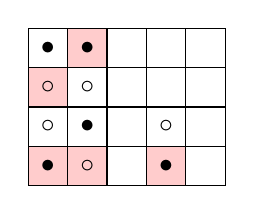
\begin{tikzpicture}

				\node [draw, fill=red!20, minimum width=0.5cm, minimum height=0.5cm] at (0, 0) {$\bullet$};
				\node [draw, fill=red!20, minimum width=0.5cm, minimum height=0.5cm] at (0.5, 0) {$\circ$};
				\node [draw, minimum width=0.5cm, minimum height=0.5cm] at (1.0, 0) {};
				\node [draw, fill=red!20, minimum width=0.5cm, minimum height=0.5cm] at (1.5, 0) {$\bullet$};
				\node [draw, minimum width=0.5cm, minimum height=0.5cm] at (2.0, 0) {};


				\node [draw, minimum width=0.5cm, minimum height=0.5cm] at (0, 0.5) {$\circ$};
				\node [draw, minimum width=0.5cm, minimum height=0.5cm] at (0.5, 0.5) {$\bullet$};
				\node [draw, minimum width=0.5cm, minimum height=0.5cm] at (1.0, 0.5) {};
				\node [draw, minimum width=0.5cm, minimum height=0.5cm] at (1.5, 0.5) {$\circ$};
				\node [draw, minimum width=0.5cm, minimum height=0.5cm] at (2.0, 0.5) {};


				\node [draw, fill=red!20, minimum width=0.5cm, minimum height=0.5cm] at (0, 1) {$\circ$};
				\node [draw, minimum width=0.5cm, minimum height=0.5cm] at (0.5, 1) {$\circ$};
				\node [draw, minimum width=0.5cm, minimum height=0.5cm] at (1.0, 1) {};
				\node [draw, minimum width=0.5cm, minimum height=0.5cm] at (1.5, 1) {};
				\node [draw, minimum width=0.5cm, minimum height=0.5cm] at (2.0, 1) {};

				\node [draw, minimum width=0.5cm, minimum height=0.5cm] at (0, 1.5) {$\bullet$};
				\node [draw, fill=red!20, minimum width=0.5cm, minimum height=0.5cm] at (0.5, 1.5) {$\bullet$};
				\node [draw, minimum width=0.5cm, minimum height=0.5cm] at (1.0, 1.5) {};
				\node [draw, minimum width=0.5cm, minimum height=0.5cm] at (1.5, 1.5) {};
				\node [draw, minimum width=0.5cm, minimum height=0.5cm] at (2.0, 1.5) {};

		\end{tikzpicture}
		\caption{An example of a board game. Cards are not represented.}
		\label{fig:board-example}
\end{figure}
\begin{figure}[ht]
		\center
		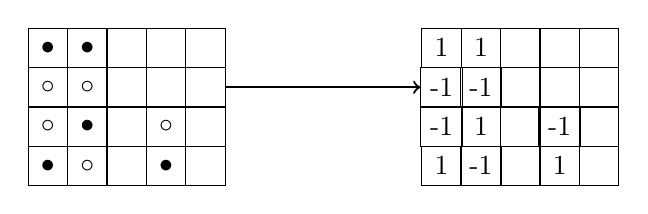
\begin{tikzpicture}

				\node [draw, minimum width=0.5cm, minimum height=0.5cm] at (0, 0) {$\bullet$};
				\node [draw, minimum width=0.5cm, minimum height=0.5cm] at (0.5, 0) {$\circ$};
				\node [draw, minimum width=0.5cm, minimum height=0.5cm] at (1.0, 0) {};
				\node [draw, minimum width=0.5cm, minimum height=0.5cm] at (1.5, 0) {$\bullet$};
				\node [draw, minimum width=0.5cm, minimum height=0.5cm] at (2.0, 0) {};


				\node [draw, minimum width=0.5cm, minimum height=0.5cm] at (0, 0.5) {$\circ$};
				\node [draw, minimum width=0.5cm, minimum height=0.5cm] at (0.5, 0.5) {$\bullet$};
				\node [draw, minimum width=0.5cm, minimum height=0.5cm] at (1.0, 0.5) {};
				\node [draw, minimum width=0.5cm, minimum height=0.5cm] at (1.5, 0.5) {$\circ$};
				\node [draw, minimum width=0.5cm, minimum height=0.5cm] at (2.0, 0.5) {};


				\node [draw, minimum width=0.5cm, minimum height=0.5cm] at (0, 1) {$\circ$};
				\node [draw, minimum width=0.5cm, minimum height=0.5cm] at (0.5, 1) {$\circ$};
				\node [draw, minimum width=0.5cm, minimum height=0.5cm] at (1.0, 1) {};
				\node [draw, minimum width=0.5cm, minimum height=0.5cm] at (1.5, 1) {};
				\node [draw, minimum width=0.5cm, minimum height=0.5cm] (A) at (2.0, 1) {};

				\node [draw, minimum width=0.5cm, minimum height=0.5cm] at (0, 1.5) {$\bullet$};
				\node [draw, minimum width=0.5cm, minimum height=0.5cm] at (0.5, 1.5) {$\bullet$};
				\node [draw, minimum width=0.5cm, minimum height=0.5cm] at (1.0, 1.5) {};
				\node [draw, minimum width=0.5cm, minimum height=0.5cm] at (1.5, 1.5) {};
				\node [draw, minimum width=0.5cm, minimum height=0.5cm] at (2.0, 1.5) {};

				\node [draw, minimum width=0.5cm, minimum height=0.5cm] at (5, 0) {1};
				\node [draw, minimum width=0.5cm, minimum height=0.5cm] at (5.5, 0) {-1};
				\node [draw, minimum width=0.5cm, minimum height=0.5cm] at (6.0, 0) {};
				\node [draw, minimum width=0.5cm, minimum height=0.5cm] at (6.5, 0) {1};
				\node [draw, minimum width=0.5cm, minimum height=0.5cm] at (7.0, 0) {};


				\node [draw, minimum width=0.5cm, minimum height=0.5cm] at (5, 0.5) {-1};
				\node [draw, minimum width=0.5cm, minimum height=0.5cm] at (5.5, 0.5) {1};
				\node [draw, minimum width=0.5cm, minimum height=0.5cm] at (6.0, 0.5) {};
				\node [draw, minimum width=0.5cm, minimum height=0.5cm] at (6.5, 0.5) {-1};
				\node [draw, minimum width=0.5cm, minimum height=0.5cm] at (7.0, 0.5) {};


				\node [draw, minimum width=0.5cm, minimum height=0.5cm] (B) at (5, 1) {-1};
				\node [draw, minimum width=0.5cm, minimum height=0.5cm] at (5.5, 1) {-1};
				\node [draw, minimum width=0.5cm, minimum height=0.5cm] at (6.0, 1) {};
				\node [draw, minimum width=0.5cm, minimum height=0.5cm] at (6.5, 1) {};
				\node [draw, minimum width=0.5cm, minimum height=0.5cm] at (7.0, 1) {};

				\node [draw, minimum width=0.5cm, minimum height=0.5cm] at (5, 1.5) {1};
				\node [draw, minimum width=0.5cm, minimum height=0.5cm] at (5.5, 1.5) {1};
				\node [draw, minimum width=0.5cm, minimum height=0.5cm] at (6.0, 1.5) {};
				\node [draw, minimum width=0.5cm, minimum height=0.5cm] at (6.5, 1.5) {};
				\node [draw, minimum width=0.5cm, minimum height=0.5cm] at (7.0, 1.5) {};

				\draw [->,thick] (A) -- (B);
		\end{tikzpicture}
		\caption{Example of transformation for the dot player based on the board in Figure~\ref{fig:board-example}.}
		\label{fig:dot-representation}
\end{figure}
\begin{figure}[ht]
		\center
		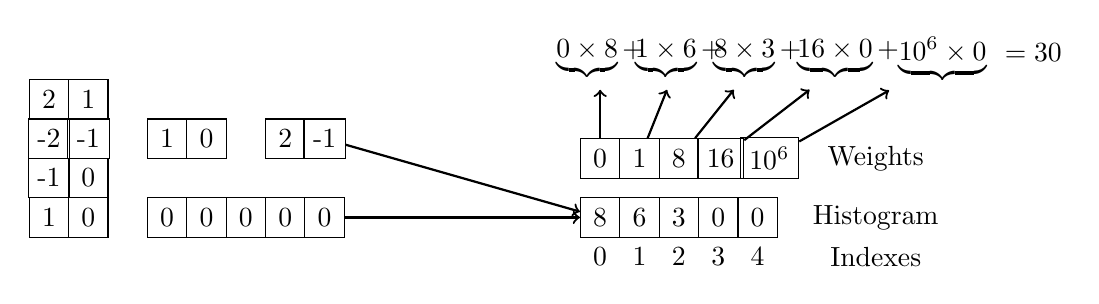
\begin{tikzpicture}

				\node [draw, minimum width=0.5cm, minimum height=0.5cm] at (0, 0) {1};
				\node [draw, minimum width=0.5cm, minimum height=0.5cm] at (0.5, 0) {0};
				\node [draw, minimum width=0.5cm, minimum height=0.5cm] at (0, 0.5) {-1};
				\node [draw, minimum width=0.5cm, minimum height=0.5cm] at (0.5, 0.5) {0};
				\node [draw, minimum width=0.5cm, minimum height=0.5cm] at (0, 1) {-2};
				\node [draw, minimum width=0.5cm, minimum height=0.5cm] at (0.5, 1) {-1};
				\node [draw, minimum width=0.5cm, minimum height=0.5cm] at (0, 1.5) {2};
				\node [draw, minimum width=0.5cm, minimum height=0.5cm] at (0.5, 1.5) {1};


				\node [draw, minimum width=0.5cm, minimum height=0.5cm] at (1.5, 0) {0};
				\node [draw, minimum width=0.5cm, minimum height=0.5cm] at (2.0, 0) {0};
				\node [draw, minimum width=0.5cm, minimum height=0.5cm] at (2.5, 0) {0};
				\node [draw, minimum width=0.5cm, minimum height=0.5cm] at (3.0, 0) {0};
				\node [draw, minimum width=0.5cm, minimum height=0.5cm] (C1) at (3.5, 0) {0};

				\node [draw, minimum width=0.5cm, minimum height=0.5cm] at (1.5, 1) {1};
				\node [draw, minimum width=0.5cm, minimum height=0.5cm] at (2.0, 1) {0};

				\node [draw, minimum width=0.5cm, minimum height=0.5cm] at (3.0, 1) {2};
				\node [draw, minimum width=0.5cm, minimum height=0.5cm] (C0) at (3.5, 1) {-1};


				\node [draw, minimum width=0.5cm, minimum height=0.5cm] (H0) at (7.0, 0) {8};
				\node [draw, minimum width=0.5cm, minimum height=0.5cm] at (7.5, 0) {6};
				\node [draw, minimum width=0.5cm, minimum height=0.5cm] at (8.0, 0) {3};
				\node [draw, minimum width=0.5cm, minimum height=0.5cm] at (8.5, 0) {0};
				\node [draw, minimum width=0.5cm, minimum height=0.5cm] at (9.0, 0) {0};

				\node [draw, minimum width=0.5cm, minimum height=0.5cm] (W0) at (7.0, 0.75) {0};
				\node [draw, minimum width=0.5cm, minimum height=0.5cm] (W1) at (7.5, 0.75) {1};
				\node [draw, minimum width=0.5cm, minimum height=0.5cm] (W2) at (8.0, 0.75) {8};
				\node [draw, minimum width=0.5cm, minimum height=0.5cm] (W3) at (8.53, 0.75) {16};
				\node [draw, minimum width=0.5cm, minimum height=0.5cm] (W4) at (9.15, 0.75) {$10^6$};
				\node at (10.5, 0.75) {Weights};
				\node at (10.5, 0) {Histogram};
				\node at (10.5, -0.5) {Indexes};

				\node at (7.0, -0.5) {0};
				\node at (7.5, -0.5) {1};
				\node at (8.0, -0.5) {2};
				\node at (8.5, -0.5) {3};
				\node at (9.0, -0.5) {4};

				\node (ID0) at (7.0, 2) {$\underbrace{0\times8} + $};
				\node (ID1) at (8.0, 2) {$\underbrace{1\times6} +$};
				\node (ID2) at (9.0, 2) {$\underbrace{8\times3} +$};
				\node (ID3) at (10.15, 2) {$\underbrace{16\times0} +$};
				\node (ID4) at (11.35, 2) {$\underbrace{10^6 \times 0}$};
				\node (ID5) at (12.5, 2.10) {$ = 30$};

				\draw [->,thick] (W0) -- (ID0);
				\draw [->,thick] (W1) -- (ID1);
				\draw [->,thick] (W2) -- (ID2);
				\draw [->,thick] (W3) -- (ID3);
				\draw [->,thick] (W4) -- (ID4);

				
				\draw [->,thick] (C0) -- (H0);
				\draw [->,thick] (C1) -- (H0);
		\end{tikzpicture}
		\caption{The four matrices obtained after applying the four masks on the matrix that represent the dot, in Figure~\ref{fig:dot-representation}.
						This Figure also represents the conversion to an histogram and how this histogram is used to find the heuristic value for the dot player.}
		\label{fig:convolution-results}
\end{figure}

\clearpage
\subsection{Vspace}
\label{sec:vspace}
The goal of the Vspace heuristic is to give value to empty
cells in addition to counting rows of similar
symbols. Similarly to the previous heuristic,
Vspace count the size of the lines, but for every
line connected to an empty cell, it uses the
size of this line as a value for the empty cell.

Figure~\ref{fig:dot-vspace} and
Figure~\ref{fig:color-vspace} give examples on
how the spaces are valued for both players, based
on the board at Figure~\ref{fig:board-example}.
Figure~\ref{fig:color-vspace} shows that even if
the line is split in two with an empty cell in the
middle, the combine value of both side gives the
value of the space. This is the reason why the two
3-values appears even though there is no line of
three.

Possible value for spaces range from 0 to 4 and
higher values are downed to 4. When multiple lines
are connected to an empty cell, the cell receives
the maximum value from them. The heuristic split the
space in two categories: the space available in
the next turn and the spaces too high to be reach
with one card.

Finally, an histogram for each category is made and
each value is multiplied by a weight then summed.
Note that the two categories have different
weights, because a space connected to a line of
three symboles does not hold the same value if you
can play on it on the next turn or not.
\begin{figure}[ht]
		\center
		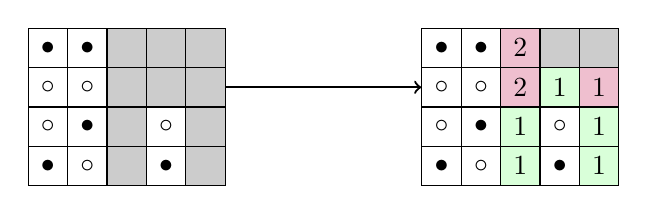
\begin{tikzpicture}

				\node [draw, minimum width=0.5cm, minimum height=0.5cm] at (0, 0) {$\bullet$};
				\node [draw, minimum width=0.5cm, minimum height=0.5cm] at (0.5, 0) {$\circ$};
				\node [draw, fill=black!20, minimum width=0.5cm, minimum height=0.5cm] at (1.0, 0) {};
				\node [draw, minimum width=0.5cm, minimum height=0.5cm] at (1.5, 0) {$\bullet$};
				\node [draw, fill=black!20, minimum width=0.5cm, minimum height=0.5cm] at (2.0, 0) {};


				\node [draw, minimum width=0.5cm, minimum height=0.5cm] at (0, 0.5) {$\circ$};
				\node [draw, minimum width=0.5cm, minimum height=0.5cm] at (0.5, 0.5) {$\bullet$};
				\node [draw, fill=black!20, minimum width=0.5cm, minimum height=0.5cm] at (1.0, 0.5) {};
				\node [draw, minimum width=0.5cm, minimum height=0.5cm] at (1.5, 0.5) {$\circ$};
				\node [draw, fill=black!20, minimum width=0.5cm, minimum height=0.5cm] at (2.0, 0.5) {};


				\node [draw, minimum width=0.5cm, minimum height=0.5cm] at (0, 1) {$\circ$};
				\node [draw, minimum width=0.5cm, minimum height=0.5cm] at (0.5, 1) {$\circ$};
				\node [draw, fill=black!20, minimum width=0.5cm, minimum height=0.5cm] at (1.0, 1) {};
				\node [draw, fill=black!20, minimum width=0.5cm, minimum height=0.5cm] at (1.5, 1) {};
				\node [draw, fill=black!20, minimum width=0.5cm, minimum height=0.5cm] (A) at (2.0, 1) {};

				\node [draw, minimum width=0.5cm, minimum height=0.5cm] at (0, 1.5) {$\bullet$};
				\node [draw, minimum width=0.5cm, minimum height=0.5cm] at (0.5, 1.5) {$\bullet$};
				\node [draw, fill=black!20, minimum width=0.5cm, minimum height=0.5cm] at (1.0, 1.5) {};
				\node [draw, fill=black!20, minimum width=0.5cm, minimum height=0.5cm] at (1.5, 1.5) {};
				\node [draw, fill=black!20, minimum width=0.5cm, minimum height=0.5cm] at (2.0, 1.5) {};

				%------
				\node [draw, minimum width=0.5cm, minimum height=0.5cm] at (5, 0) {$\bullet$};
				\node [draw, minimum width=0.5cm, minimum height=0.5cm] at (5.5, 0) {$\circ$};
				\node [draw, fill=green!15, minimum width=0.5cm, minimum height=0.5cm] at (6.0, 0) {1};
				\node [draw, minimum width=0.5cm, minimum height=0.5cm] at (6.5, 0) {$\bullet$};
				\node [draw, fill=green!15, minimum width=0.5cm, minimum height=0.5cm] at (7.0, 0) {1};


				\node [draw, minimum width=0.5cm, minimum height=0.5cm] at (5, 0.5) {$\circ$};
				\node [draw, minimum width=0.5cm, minimum height=0.5cm] at (5.5, 0.5) {$\bullet$};
				\node [draw, fill=green!15, minimum width=0.5cm, minimum height=0.5cm] at (6.0, 0.5) {1};
				\node [draw, minimum width=0.5cm, minimum height=0.5cm] at (6.5, 0.5) {$\circ$};
				\node [draw, fill=green!15, minimum width=0.5cm, minimum height=0.5cm] at (7.0, 0.5) {1};


				\node [draw, minimum width=0.5cm, minimum height=0.5cm] (B) at (5, 1) {$\circ$};
				\node [draw, minimum width=0.5cm, minimum height=0.5cm] at (5.5, 1) {$\circ$};
				\node [draw, fill=purple!25, minimum width=0.5cm, minimum height=0.5cm] at (6.0, 1) {2};
				\node [draw, fill=green!15, minimum width=0.5cm, minimum height=0.5cm] at (6.5, 1) {1};
				\node [draw, fill=purple!25, minimum width=0.5cm, minimum height=0.5cm] at (7.0, 1) {1};

				\node [draw, minimum width=0.5cm, minimum height=0.5cm] at (5, 1.5) {$\bullet$};
				\node [draw, minimum width=0.5cm, minimum height=0.5cm] at (5.5, 1.5) {$\bullet$};
				\node [draw, fill=purple!25, minimum width=0.5cm, minimum height=0.5cm] at (6.0, 1.5) {2};
				\node [draw, fill=black!20, minimum width=0.5cm, minimum height=0.5cm] at (6.5, 1.5) {};
				\node [draw, fill=black!20, minimum width=0.5cm, minimum height=0.5cm] at (7.0, 1.5) {};

				\draw [->,thick] (A) -- (B);
		\end{tikzpicture}
		\caption{Example of the Vspace process for the
		dot player based on the board in
		Figure~\ref{fig:board-example}. the grey cells
		represent cells that contain nothing
		interesting. On the right board, green cells
		are spaces available for the next turn and
		purple cells are spaces that need at least two
		cards to be filled.}
		\label{fig:dot-vspace}
\end{figure}
\begin{figure}[ht]
		\center
		\begin{tikzpicture}

				\node [draw, fill=red!20, minimum width=0.5cm, minimum height=0.5cm] at (0, 0) {};
				\node [draw, fill=red!20, minimum width=0.5cm, minimum height=0.5cm] at (0.5, 0) {};
				\node [draw, fill=black!20, minimum width=0.5cm, minimum height=0.5cm] at (1.0, 0) {};
				\node [draw, fill=red!20, minimum width=0.5cm, minimum height=0.5cm] at (1.5, 0) {};
				\node [draw, fill=black!20, minimum width=0.5cm, minimum height=0.5cm] at (2.0, 0) {};


				\node [draw, minimum width=0.5cm, minimum height=0.5cm] at (0, 0.5) {};
				\node [draw, minimum width=0.5cm, minimum height=0.5cm] at (0.5, 0.5) {};
				\node [draw, fill=black!20, minimum width=0.5cm, minimum height=0.5cm] at (1.0, 0.5) {};
				\node [draw, minimum width=0.5cm, minimum height=0.5cm] at (1.5, 0.5) {};
				\node [draw, fill=black!20, minimum width=0.5cm, minimum height=0.5cm] at (2.0, 0.5) {};


				\node [draw, fill=red!20, minimum width=0.5cm, minimum height=0.5cm] at (0, 1) {};
				\node [draw, minimum width=0.5cm, minimum height=0.5cm] at (0.5, 1) {};
				\node [draw, fill=black!20, minimum width=0.5cm, minimum height=0.5cm] at (1.0, 1) {};
				\node [draw, fill=black!20, minimum width=0.5cm, minimum height=0.5cm] at (1.5, 1) {};
				\node [draw, fill=black!20, minimum width=0.5cm, minimum height=0.5cm] at (2.0, 1) {};

				\node [draw, minimum width=0.5cm, minimum height=0.5cm] at (0, 1.5) {};
				\node [draw, fill=red!20, minimum width=0.5cm, minimum height=0.5cm] at (0.5, 1.5) {};
				\node [draw, fill=black!20, minimum width=0.5cm, minimum height=0.5cm] at (1.0, 1.5) {};
				\node [draw, fill=black!20, minimum width=0.5cm, minimum height=0.5cm] at (1.5, 1.5) {};
				\node [draw, fill=black!20, minimum width=0.5cm, minimum height=0.5cm] at (2.0, 1.5) {};

				%------
				\node [draw, fill=red!20, minimum width=0.5cm, minimum height=0.5cm] at (5, 0) {};
				\node [draw, fill=red!20, minimum width=0.5cm, minimum height=0.5cm] at (5.5, 0) {};
				\node [draw, fill=green!15, minimum width=0.5cm, minimum height=0.5cm] at (6.0, 0) {3};
				\node [draw, fill=red!20, minimum width=0.5cm, minimum height=0.5cm] at (6.5, 0) {};
				\node [draw, fill=green!15, minimum width=0.5cm, minimum height=0.5cm] at (7.0, 0) {1};


				\node [draw, minimum width=0.5cm, minimum height=0.5cm] at (5, 0.5) {};
				\node [draw, minimum width=0.5cm, minimum height=0.5cm] at (5.5, 0.5) {};
				\node [draw, fill=green!15, minimum width=0.5cm, minimum height=0.5cm] at (6.0, 0.5) {3};
				\node [draw, minimum width=0.5cm, minimum height=0.5cm] at (6.5, 0.5) {};
				\node [draw, fill=green!15, minimum width=0.5cm, minimum height=0.5cm] at (7.0, 0.5) {1};


				\node [draw, fill=red!20, minimum width=0.5cm, minimum height=0.5cm] (B) at (5, 1) {};
				\node [draw, minimum width=0.5cm, minimum height=0.5cm] at (5.5, 1) {};
				\node [draw, fill=purple!25, minimum width=0.5cm, minimum height=0.5cm] at (6.0, 1) {1};
				\node [draw, fill=green!15, minimum width=0.5cm, minimum height=0.5cm] at (6.5, 1) {1};
				\node [draw, fill=purple!25, minimum width=0.5cm, minimum height=0.5cm] at (7.0, 1) {1};

				\node [draw, minimum width=0.5cm, minimum height=0.5cm] at (5, 1.5) {};
				\node [draw, fill=red!20, minimum width=0.5cm, minimum height=0.5cm] at (5.5, 1.5) {$\bullet$};
				\node [draw, fill=purple!25, minimum width=0.5cm, minimum height=0.5cm] at (6.0, 1.5) {2};
				\node [draw, fill=black!20, minimum width=0.5cm, minimum height=0.5cm] at (6.5, 1.5) {};
				\node [draw, fill=black!20, minimum width=0.5cm, minimum height=0.5cm] at (7.0, 1.5) {};

				\draw [->,thick] (A) -- (B);
		\end{tikzpicture}
		\caption{Example of the Vspace process for the
		color player based on the board in
		Figure~\ref{fig:board-example}. the grey cells
		represent cells that contain nothing
		interesting. On the right board, green cells
		are spaces available for the next turn and
		purple cells are spaces that need at least two
		cards to be filled.}
		\label{fig:color-vspace}
\end{figure}
\clearpage
\section{Difficulties}
\subsection{Slowness}
The biggest difficulty encountered during this
project was the slowness of python. In the early
stage of the project, the code was
too ineficient and could not check more than one
move in advance within the limit of three seconds. 

The \textit{cProfile} python module is a module
that helps to profile python code. In particular,
it give the amount of time spent in each function
called. This profiler was used to locate the most
time consumming function, then I rely on this information to
restructure the code into better object structure.

However, the result were hardly perceivable and
the code was still too slow for competetive use.
Therefore, I turn to two scientific python
libraries: Numpy and Scipy. Using functions from
these libraries slightly improved the performance
because they were built-in functions. In python,
built-in functions are C functions compiled into a
python module and called from python script.

Finally, to reach a decent executing time, 
one more step was taken and a python module writen
in C was developed.
Figure~\ref{fig:performance-magic} show the
evolution of the performances as the most time
consuming function were adapted to call the
module. However, the python code remains and it is
executed by default. 
Figure~\ref{fig:performance-magic} shows that the
MinMax algorithm is able to check four moves in
advance after half of the key part used the
module.

\begin{figure}
		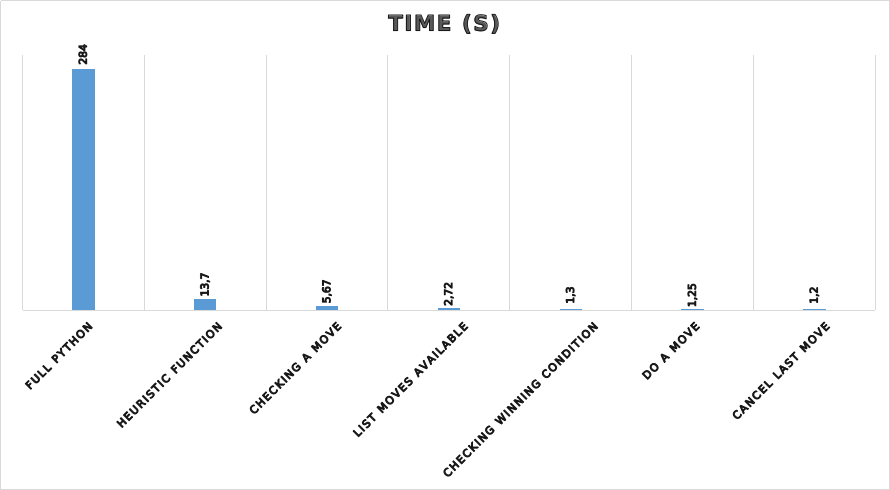
\includegraphics[width=\textwidth]{perfromances.png}
		\caption{The amount of time (in second) taken
		to run the MinMax algorithm on a board with the
		card "5 B 1" already played. The MinMax
		algorithm checked up to 4 moves in advance and
		it used the Vspace heuristic described in
		Section~\ref{sec:vspace}. The left column
		shows the full python execution time (more
		than 4 minutes) and the other columns show the
		execution time as part of the code start using
		the C module. The third column from the left,
		"checking a move", indicate the time taken
		when the heuristic function and the function
		that check the moves use both the C module.}
		\label{fig:performance-magic}
\end{figure}

\begin{itemize}
		\item Version changing between Python 3.7.2 and 3.5.1 (serialization of regex)
\end{itemize}
\section{Analyze}
\begin{itemize}
		\item How is the pruning depth 3 with a
				recycling moves: no prun = 26s, prun=0.3s.
		\item How are the performance at the tournament.
\end{itemize}

\section{A Subsection Sample}
Please note that the first paragraph of a section or subsection is
not indented. The first paragraph that follows a table, figure,
equation etc. does not need an indent, either.

Subsequent paragraphs, however, are indented.

\subsubsection{Sample Heading (Third Level)} Only two levels of
headings should be numbered. Lower level headings remain unnumbered;
they are formatted as run-in headings.

\paragraph{Sample Heading (Fourth Level)}
The contribution should contain no more than four levels of
headings. Table~\ref{tab1} gives a summary of all heading levels.

\begin{table}
\caption{Table captions should be placed above the
tables.}\label{tab1}
\begin{tabular}{|l|l|l|}
\hline
Heading level &  Example & Font size and style\\
\hline
Title (centered) &  {\Large\bfseries Lecture Notes} & 14 point, bold\\
1st-level heading &  {\large\bfseries 1 Introduction} & 12 point, bold\\
2nd-level heading & {\bfseries 2.1 Printing Area} & 10 point, bold\\
3rd-level heading & {\bfseries Run-in Heading in Bold.} Text follows & 10 point, bold\\
4th-level heading & {\itshape Lowest Level Heading.} Text follows & 10 point, italic\\
\hline
\end{tabular}
\end{table}


\noindent Displayed equations are centered and set on a separate
line.
\begin{equation}
x + y = z
\end{equation}
Please try to avoid rasterized images for line-art diagrams and
schemas. Whenever possible, use vector graphics instead (see
Fig.~\ref{fig1}).

\begin{figure}
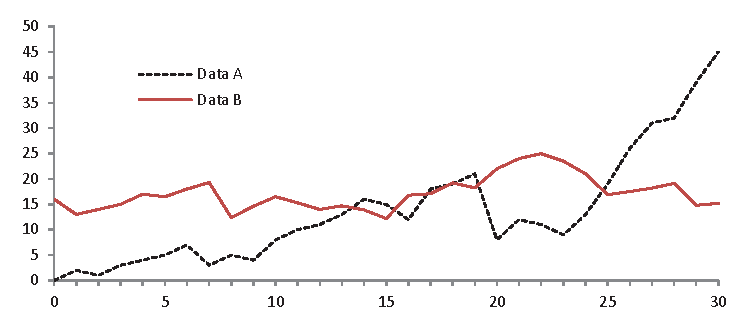
\includegraphics[width=\textwidth]{fig1.eps}
\caption{A figure caption is always placed below the illustration.
Please note that short captions are centered, while long ones are
justified by the macro package automatically.} \label{fig1}
\end{figure}

\begin{theorem}
This is a sample theorem. The run-in heading is set in bold, while
the following text appears in italics. Definitions, lemmas,
propositions, and corollaries are styled the same way.
\end{theorem}
%
% the environments 'definition', 'lemma', 'proposition', 'corollary',
% 'remark', and 'example' are defined in the LLNCS documentclass as well.
%
\begin{proof}
Proofs, examples, and remarks have the initial word in italics,
while the following text appears in normal font.
\end{proof}
For citations of references, we prefer the use of square brackets
and consecutive numbers. Citations using labels or the author/year
convention are also acceptable. The following bibliography provides
a sample reference list with entries for journal
articles~\cite{ref1}, an LNCS chapter~\cite{ref2}, a
book~\cite{ref1}, proceedings without editors~\cite{ref1},
and a homepage~\cite{ref_2}. Multiple citations are grouped
\cite{ref1,ref2}.
% ---- Bibliography ----
%
% BibTeX users should specify bibliography style 'splncs04'.
% References will then be sorted and formatted in the correct style.
%
% \bibliographystyle{splncs04}
% \bibliography{mybibliography}
%
\bibliographystyle{splncs04}
\bibliography{paper}
\end{document}

% vim: tw=50 ts=2
